% Modificaciones realizadas al archivo revista_poli-01.sty
% por: LeninGF
% Fecha: 2020/04/29
% Este formato utiliza biblatex en vez de natib
% Las referencias se pueden colocar en un archivo referencias.bib
% se pueden usar los comandos \textcite, \cite
\documentclass[10.5 pt, twocolumn]{article}
\usepackage{revista_poli-01}
\usepackage{multirow}
\usepackage{ctable} %para mejorar el formato de las tablas

%titulo: [titulo corto (va en el heading)] {titulo largo (tiulo del articulo)}
\titlerevista[Preparación de Artículos para la Revista Politécnica]{Preparación de Artículos para la Revista Politécnica Utilizar Mayúsculas en cada Palabra en el Caso del Título}%el corchete se puede omitir, pero si el título es muy grande, se puede usar este para poner un título más corto en los encabezados
\newcommand{\tituloingles}{ Title of Manuscript} %titulo del articulo en inglés
\newcommand{\correoautor}{\footnotesize Colocar el correo electrónico del autor de correspondencia} %correo del autor principal

\authorrevista[1][]{Apellido, Nombre}
\authorrevista[2][]{Apellido, Nombre}
\authorrevista[3][]{Apellido, Nombre}
\authorrevista[3][]{Apellido, Nombre}
%
\institucionmail[1][]{Institución, Departamento o Facultad del Autor Principal, Ciudad, País}{} 
\institucionmail[2]{Institución, Departamento o Facultad del Autor 2, Ciudad, País}{}
\institucionmail[3]{Institución, Departamento o Facultad del Autor 3 y 4, Ciudad, País}{}


\sethdrevista

\makeatletter
\def\blfootnote{\xdef\@thefnmark{}\@footnotetext}%con esto, definimos el comando \blfootnote{texto de pie de pagina} que genera un pie de pagina sin numeracion.
\makeatother

%\renewcommand\abstractname{\vspace{-\baselineskip}}

\fancypagestyle{plain}{
\fancyhead[R]{ }
\fancyhead[L]{ }
\fancyfoot[R]{ }
\fancyfoot[L]{{\rule[1.5cm]{5.2cm}{.4pt} \\[-1.5cm]\scriptsize \correoautor} }
\renewcommand{\headrulewidth}{0.5pt}
}
\pagestyle{fancy}


\begin{document}

\twocolumn[{

\maketitlerevista

\renewcommand\abstractname{\vspace{-2\baselineskip}}

\hspace*{0.05\linewidth}\begin{minipage}{0.9\linewidth}
\begin{resumen}
\textbf{Resumen:} Las siguientes instrucciones establecen las pautas para la preparación de artículos para la Revista Politécnica. Los artículos pueden ser escritos en español o en inglés, pero tendrán un resumen de máximo 250 palabras en los dos idiomas. Los autores pueden hacer uso de este archivo (.tex) como una plantilla para componer su artículo si están utilizando  \LaTeX $  2\epsilon$. Caso contrario, este documento puede ser utilizado como una guía de instrucciones. El número mínimo de páginas será 6 y el máximo 15,  Para el envío de los artículos, los autores deben seguir las instrucciones colocadas en el sistema de recepción de artículos del sitio web de la Revista Politécnica (\url{revistapolitecnica.epn.edu.ec}). En caso de que su artículo sea en inglés colocar el título y el resumen en los dos idiomas.  

\palabrasclavesrevista{Incluir una lista de 3-6 palabras clave.}
\end{resumen}
\vspace*{-0.3cm}
\begin{center}
\LARGE\bf \tituloingles
\end{center} 
\vspace*{-0.3cm}
\begin{abstract}
\textbf{Abstract:} These instructions give you guidelines for preparing papers for EPN Journal. Papers can be written in Spanish or English; however, an abstract of maximum 250 words and written in both languages is required. Use this document (.tex) as a template to compose your paper if you are using \LaTeX $2\epsilon$. Otherwise, use this document as an instruction set. The minimum number of pages will be 6 and the maximum will be 15. For submission guidelines, follow instructions on paper submission system from the EPN Journal website (\url{revistapolitecnica.epn.edu.ec}).

\keywordsrevista{Include a list of 3-6 keywords.}
\end{abstract}
\end{minipage}

}]

\section{SECCIÓN I}

Este documento es una plantilla para \LaTeX{} $2\varepsilon$. Si está leyendo una versión impresa de este documento, por favor descargue el archivo  electrónico, \textbf{\url{https://url.epn.edu.ec/FormatoRPLatex}} donde se encuentra la plantilla \textbf{Formato$.$tex} y la clase \textbf{revista$\_$poli-01}. Por favor, {\bf no modifique la clase y no coloque ninguna numeración de página, encabezado / pie de página en la plantilla presentada}. Utilice \textit{cursiva} o \textbf{negrita} para dar énfasis a un texto, no subrayado. En caso de que el autor desee enviar el artículo en formato Word por favor descargue el archivo desde \textbf{\url{https://url.epn.edu.ec/FormatoRPWord}} o comunicarse con la coordinación de edición (epnjournal@epn.edu.ec).

\section{SECCIÓN II}

Para las pautas de presentación, siga las instrucciones emitidas por el sistema del sitio web de la revista de la EPN. La presentación inicial debe tomar en cuenta todas las indicaciones que se presentan en la plantilla, para de esta manera tener una buena estimación de la longitud del artículo a publicarse. Además, de esta manera el esfuerzo necesario para la presentación final del manuscrito será mínimo. Como sugerencia, es importante tomar en cuenta que, el primer autor es el investigador que hizo la mayor parte del trabajo, mientras que el último autor suele ser el profesor quien es el líder intelectual y, a menudo edita y presenta el borrador final del documento. La Revista Politécnica pondrá en marcha un sistema de transferencia electrónica de derechos de autor en su momento. Por favor, ``no'' enviar formularios de derecho de autor por correo o fax. A continuación se detallan las consideraciones que se deben tener en cuenta para la presentación final del artículo.

\section{SECCIÓN III}


\subsection{Figuras, tablas y márgenes}
Todas las figuras deben ser incorporadas en la carpeta con el archivo Formato.tex. En lo posible, utilice las herramientas de conversión estándar PDF Adobe Acrobat o GhostScript que brindan mejores resultados. Es importante que todas las fuentes estén establecidas en el PDF resultante. Puede también utilizar formato png. La sugerencia es

\begin{itemize}
\item pdf: si la salida es de un programa
\item png: si es una captura de pantalla, mapa de Bits (Windows)
\end{itemize}

tome en cuenta que las figuras, dibujos, fotografías deberan tener al menos 1200 puntos (resolusión), con leyendas legibles y de tamaño adecuado. El artículo debe contener entre tablas y figuras un máximo de 10. \\

Las etiquetas de los ejes de las figuras son a menudo una fuente de confusión. Utilice las palabras en lugar de símbolos. Por ejemplo, escriba la cantidad ``Magnetización'', o ``Magnetización M'' no sólo ``M''.\\

Las figuras y tablas deben estar en la parte superior e inferior de las columnas. Evite colocarlas en medio de las columnas. Las figuras y tablas grandes pueden extenderse a lo largo de ambas columnas. Las leyendas de las figuras deben estar centradas debajo de las figuras, los títulos de las tablas deben estar centrados arriba. Evite colocar figuras y tablas antes de su primera mención en el texto. Para la mención de figuras, tablas o ecuaciones utilice las palabras completas con la primera letra en mayúscula, por ejemplo ``Figura \ref{fig:01}''. Utilice etiquetas para referenciar sus tablas y figuras. \\

Coloque las unidades entre paréntesis. No etiquete los ejes sólo con unidades. Por ejemplo, escriba ``Magnetización (A/m)'' o ``Magnetización (Am$^{-1}$)'', no sólo ``Magnetización A/m''. No etiquete los ejes con una relación de cantidades y unidades. Por ejemplo, escriba ``Temperatura ($^\circ$K)'', no ``Temperatura $^\circ$K''.\\

Los multiplicadores pueden ser especialmente confusos. Escriba ``Magnetización (kA/m)'' o ``Magnetización (10$^3$ A/m)''. No escriba ``Magnetización (A/m)$\times$ 1000'' porque el lector no sabrá si la etiqueta del eje de arriba significa 16000 A/m o 0.016 A/m.\\
% h!t!b!
\begin{figure}[htbp]
{\centering
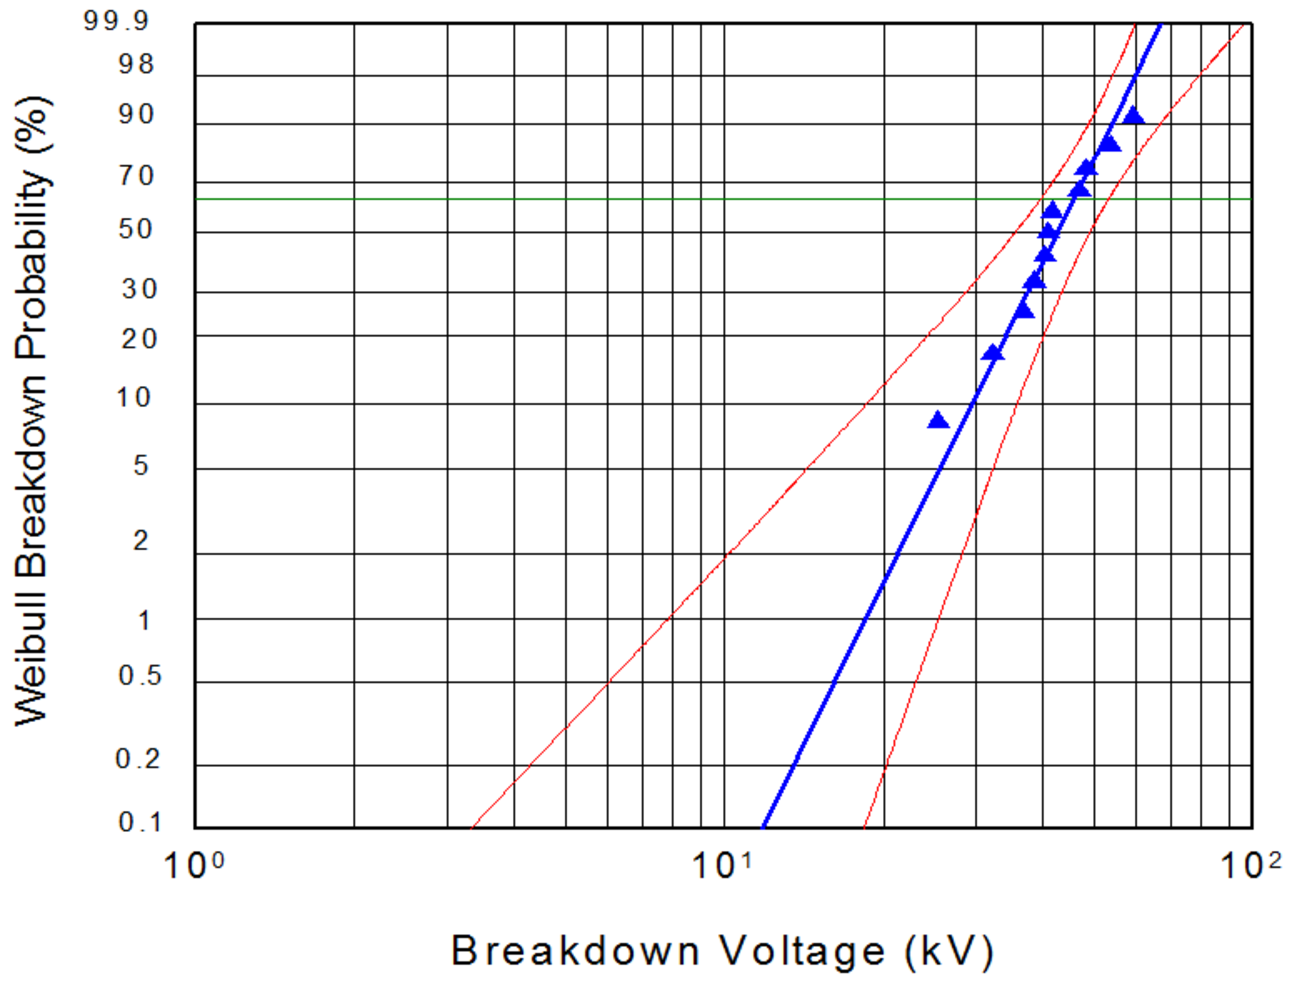
\includegraphics[width=0.40\textwidth]{fig1.pdf} \\[-0.4cm]
\captionof{figure}{{\it Distribución} Weibull de 60 Hz voltajes de ruptura 11 cables $\alpha = 45.9$ kV pico $\beta = 5.08$. Intervalo de Confidencia 95\%.}
\label{fig:01}
}
\end{figure}

Los autores deben trabajar activamente con los márgenes solicitados. Los documentos de la revista serán marcados con los datos del registro de la revista y paginados para su inclusión en la edición final. Si la sangría de los márgenes en su manuscrito no es correcta, se le pedirá que lo vuelva a presentar y esto, podría retrasar la preparación final durante el proceso de edición. Ejemplo de cita y tabla: \textcite{young1964synthetic} en su artículo publicó datos experimentales de distintas moléculas donde \ldots. \\

%Ejemplo de tabla, en lo posible no modificar los saltos entre líneas 
% h!
\begin{table}[!ht]
    \footnotesize %tamaño de letra en la tabla (no modificar)
        \begin{center}
            \caption{Constantes moleculares \\[-0.3cm]} %el caption tiene su propio tamaño de letra - no cambiarlo
            \begin{tabular}{c c c c}
                \hline
                \\[-0.3cm]
                \multirow{2}{*}{{\bf Molécula}} &  {\bf Masa}  &  {\bf Elasticidad}  &   {\bf Energía de Disociación}  \\ [-1pt]
                & $ {\mu (10^ {-27} Kg)}$ & $ k_e (N/m)$ & ${ D_e (10^ {-19} \text{J})}$ \\[1pt]
                \hline 
                \\[-0.3cm]
                 HF & $1,589$ & $800$ & $9,812$ \\ [-1pt]
                 HCl & $1,623$ & $480$ & $7,100$ \\ [-1pt]
                 HBr & $1,653$ &  $300$ & $5,725$ \\  [-1.5pt]
                \hline
            \end{tabular} 
            \label{fig1-constantes-moleculares}
        \end{center}
\end{table}
\vspace{1cm} %puede modifircar este espaciado 

Otro ejemplo, en la siguiente tabla todos los datos están en $cm$
%Ejemplo de tabla, en lo posible no modificar los saltos entre líneas 
\begin{table}[!htb]
    \footnotesize %tamaño de letra en la tabla (no modificar)
    \begin{center}
        \caption{Márgenes de páginas para formato en Word \\[-0.3cm]} %el caption tiene su propio tamaño de letra - no cambiarlo
        \begin{tabular}{c c c c}
            \hline\\[-0.3cm] 
             \multirow{2}{*}{{\bf Página}} &  \multirow{2}{*}{\bf Superior} &  \multirow{2}{*}{\bf Inferior} & \bf Izquierda/ \\  [-1pt]
             & & &\bf Derecha \\ [-1.5pt]
             \hline
             \\ [-0.3cm]
             Primera & $2,0$ & $2,5$ & $1,5$ \\ [-1pt]
             Resto & $2,0$ & $2,5$ & $1,5$ \\ [-1.5pt]
             \hline
        \end{tabular} 
        \label{fig2-medidas}
    \end{center}
\end{table}

\subsection{Ecuaciones}
La clase de esta plantilla tiene agregada los paquetes amsmath y amssymb. las ecuaciones sin numeración puede escribirlas entre signos de \$ \$ (mirar el archivo.tex) para ecuaciones dentro del texto. Ejemplo: La ecuación del área de un círculo es $A = \pi r^2$ donde \ldots. Enumere las ecuaciones importantes. \\

Para ecuaciones importantes utilice $\setminus$label$\lbrace \text{etiqueta}\rbrace$ para etiquetar a sus ecuaciones.  Luego las mismas serán llamadas mediante $\setminus$eqref $\lbrace$etiqueta$\rbrace$. 

\begin{equation}
    \int _0  ^{r_2} F(r,\varphi ) dr d\varphi=[\sigma r_2 /(2 \mu _0)]
    \label{eq-1}
\end{equation}

Asegúrese de que los símbolos en su ecuación han sido definidos antes de que aparezcan en la ecuación o inmediatamente después. Ponga en cursiva los símbolos ($T$ podría referirse a la temperatura, pero T es la unidad tesla). Para referirse a la ecuación se escribe por ejemplo ``Ecuación \eqref{eq-1} "

\section{UNIDADES}

Utilice el SI como unidades primarias. Otras unidades pueden ser utilizadas como unidades secundarias (en paréntesis). Por ejemplo, escriba ``15 Gb/cm2 (100 $Gb/in^2$)''. Evite combinar las unidades del SI y CGS, como la corriente en amperios y el campo magnético en oerstedios. Esto a menudo lleva a confusión porque las ecuaciones no cuadran dimensionalmente. Si tiene que usar unidades mixtas, aclare las unidades para cada cantidad en una ecuación.\\

Por ejemplo, en el SI la unidad de fuerza de campo magnético H es A / m. Sin embargo, si desea utilizar unidades de T, o bien se refiere a la densidad de flujo magnético B o la fuerza del campo magnético simbolizadas como $\mu_0$H. Use un punto en el centro para separar las unidades compuestas, por ejemplo, ``$A\cdot m^2$''.
\subsection{Abreviaturas y Siglas}

Defina las abreviaciones y acrónimos la primera vez que se utilizan en el texto, incluso después de que ya han sido definidos en el resumen. No utilice abreviaturas en el título a menos que sea inevitable.

\subsection{Otras recomendaciones}

\begin{itemize}
\item 	Para expresar valores decimales se usarán comas, por ejemplo $3,45$. Use un cero antes del decimal.
\item 	Se incluirá un espacio entre números para indicar los valores de miles, por ejemplo 463 690.
\item Utilice notación científica para expresar números con más de 3 cifras hacia la derecha o izquierda, es decir, mayores a $2,50\times 10^{+5}$ o menores a $4,8\times 10^{-3}.$
\item Finalmente, de ser necesario y de manera opcional, se pueden incluir conclusiones, recomendaciones y agradecimiento.
\end{itemize}

\section{Sobre las Referencias}
La lista de referencias \textbf {deben estar en Formato APA ordenada alfabéticamente} de acuerdo con el primer autor de la lista de referencia. El agregado et al no debe ir en cursiva. Por favor nótese que todas las referencias listadas aquí deben estar directamente citadas en el cuerpo del texto usando Apellido (año). Ejemplo, \cite{chen1990linear} o \cite{trevino2016managing} y para varios \cite{Falconi2020, duchesne2018educational, sainaghi2008strategic, harrison2005development}. Las notas al pie deben evitarse en la medida de lo posible. En en archivo .txt estan comentados algunos ejemplos de referencias. Para la bibliografía en el archivo.txt se sigue el siguiente formato dependiendo si es artículo, libro, etc.

$\setminus$bibitem [autor-principal  (año) autor2 and autor3 ]$\lbrace$ numero-referencia$\rbrace$autor-principla, autor2 y autor3. (año). \dots \\

El artículo debe contener un mínimo de 6 referencias. En el archivo .txt se puede revisar algunos ejemplos de citas. 

\printbibliography[title={Referencias}]


\end{document}
